\documentclass[11pt,twoside]{article}
\usepackage[preprint]{jmlr2e}
\usepackage{amsmath,mathtools,booktabs,array}
\usepackage{tikz,pgfplots}
\usetikzlibrary{arrows.meta,positioning,fit}
\pgfplotsset{compat=1.18}
\newcommand{\R}{\mathbb R}
\newcommand{\Q}{\mathbb Q}
\newcommand{\N}{\mathbb N}
\newcommand{\Sym}{\operatorname{Sym}}
\newcommand{\supp}{\operatorname{supp}}
\newcommand{\rank}{\operatorname{rank}}
\newcommand{\diag}{\operatorname{diag}}
\newcommand{\tr}{\operatorname{tr}}
\newcommand{\spanof}{\operatorname{span}}
\newcommand{\odeco}{\mathcal O_n}
\newcommand{\calF}{\mathcal F}
\newcommand{\calC}{\mathcal C}
\newcommand{\calS}{\mathcal S}
\newcommand{\norm}[1]{\lVert #1\rVert}
\newcommand{\abs}[1]{\lvert #1\rvert}
\newcommand{\ip}[2]{\langle #1,#2\rangle}
\newcommand{\one}{\mathbf 1}
\DeclareMathOperator*{\argmin}{arg\,min}
\hypersetup{
  pdftitle={Diagonal Completion: Proofs and Certificates},
  pdfauthor={Haoyi Zhang and Huaijin Ran},
  pdfsubject={Proof supplement and exact certificate semantics for diagonal completion of orthogonal tensors},
  pdfkeywords={orthogonal tensors, diagonal completion, exact certificates, identifiability}
}
\ShortHeadings{Diagonal Completion: Proofs and Certificates}{Zhang and Ran}
\firstpageno{1}

\begin{document}
\title{Diagonal Completion: Proofs and Certificates}
\author{\name Haoyi Zhang \email hyeliozhang@gmail.com \\
\addr Xi'an Jiaotong-Liverpool University
\AND
\name Huaijin Ran \email huaijin003@e.ntu.edu.sg \\
\addr Nanyang Technological University}
\maketitle
This standalone supplement contains the model, complete mathematical arguments,
worked certificates, and representation semantics. The computational checks in
this repository are finite validation, not machine-checked proofs of these general statements.
The observation basis is fixed and the class is the union of real orthogonal ranks.  In addition to the exact all-input fiber, the supplement proves the low-dimensional obstruction and the probability-one rigidity threshold for continuous odeco parameters.

\paragraph{Literature map.}
The factor-uniqueness background comes from CP identifiability and the algebraic
characterization of orthogonally decomposable tensors
\citep{bhaskara2014,boralevi2017,robeva2016,koiran2021}.
The moment-method lineage and its perturbation questions are represented by
\citet{anandkumar2014}, the block-sparse analysis of \citet{anandkumar2016},
and later orthogonal-tensor perturbation studies
\citep{luo2021,xia2019,auddy2023,yuan2026}.
Completion work addresses different masks or quantifiers: algebraic matrix
completion \citep{kiraly2015}, low-CP-rank completion
\citep{ashraphijuo2017,haselby2024}, recovery from all-distinct multilinear
entries \citep{schramm2015}, and low-rank estimation guarantees
\citep{tongwu2026}. The closest robust odeco comparison treats locally
correlated additive noise \citep{mickelin2023}, while the finite-source
interpretation below meets the higher-order factor-analysis setting of
\citet{ardiyansyah2023}. These references provide context; the proofs below
establish the fixed-basis diagonal-completion statements used by the checker.

\section{The observation model and identifiable parameters}\label{sec:model}
\subsection{Tensors, slices, and a fixed coordinate basis}
Throughout, $n\geq1$ and the base field for the mathematical statements is $\R$. A tensor $T\in\Sym^3(\R^n)$ is a real array invariant under all permutations of its indices. Its $i$th slice is the real symmetric matrix $T_i$ with $(T_i)_{pq}=T_{ipq}$. We use the Frobenius norm on the full array, counting all ordered entries, and the Euclidean norm on vectors. In particular, a two-equal-index orbit has multiplicity three and an all-distinct orbit has multiplicity six.

Define the coordinate-diagonal embedding and mixed projection by
\begin{equation}\label{eq:diagonal}
 D(x)=\sum_{i=1}^n x_i e_i^{\otimes3},\qquad
 P_{\rm mix}T=T-D((T_{111},\ldots,T_{nnn})^\top).
\end{equation}
The word ``mixed'' includes $T_{iij}$ and $T_{ijj}$ when $i\ne j$. It does not mean that all three indices must be distinct. This distinction matters: those two-equal-index entries carry the edges of our graph.

\begin{definition}[Orthogonal model]\label{def:odeco}
The class $\odeco$ consists of tensors
\begin{equation}\label{eq:odeco}
 T=\sum_{a=1}^r\lambda_a u_a^{\otimes3},\qquad
 u_a^\top u_b=\one_{a=b},\quad \lambda_a\ne0,\quad 0\le r\le n.
\end{equation}
The empty sum is the zero tensor. The model does not fix $r$. By changing the sign of $u_a$, every nonzero weight can be oriented positive.
\end{definition}
For a mixed tensor $H=P_{\rm mix}H$, the completion fiber is
\begin{equation}\label{eq:fiber-def}
 \calF(H)=\{x\in\R^n:H+D(x)\in\odeco\}.
\end{equation}
We distinguish the vector fiber from its tensor image, which is an isometric affine embedding whenever the fiber is affine. The tensor rank of a member need not be constant over that fiber.

In the exact corruption model we observe $(H,d)$, with
\begin{equation}\label{eq:exact-model}
 T^*=H+D(x^*)\in\odeco,\qquad d=x^*+e.
\end{equation}
An allowed support family $\calS$ means that $\supp(e)$ is contained in some $S\in\calS$. The values on that support are arbitrary real numbers. The cardinality model uses $\calS_s=\{S\subseteq[n]:|S|\le s\}$. This is a deterministic model: no probability of a corruption location or sign is assumed.

\subsection{A finite independent-source interpretation}
One source of~\eqref{eq:exact-model} is the third moment of
\begin{equation}\label{eq:latent}
 X=US+\varepsilon,
\end{equation}
where $U\in\R^{n\times r}$ has orthonormal columns, the coordinates of $S$ are independent and centered, and $\varepsilon$ has independent centered coordinates and is independent of $S$. Suppose third moments exist. Expanding $\mathbb E[X_iX_jX_k]$, every mixed term containing independent centered factors vanishes. Thus
\begin{equation}\label{eq:moment}
 \mathbb E[X^{\otimes3}]
 =\sum_{a=1}^r \mathbb E[S_a^3]u_a^{\otimes3}
   +D\big((\mathbb E[\varepsilon_i^3])_{i=1}^n\big).
\end{equation}
At order three, centered moments equal cumulants. The diagonal-noise cumulant model is already part of higher-order factor analysis \citep{ardiyansyah2023}; our additional restriction is orthogonality in the observed basis.

This model can have a finite latent state space. If $B$ is Bernoulli with success probability $p\in(0,1)$, then
\begin{equation}\label{eq:bernoulli}
 S=\frac{B-p}{\sqrt{p(1-p)}}
 \quad\hbox{satisfies}\quad
 \mathbb E[S]=0,\quad \mathbb E[S^2]=1,\quad
 \mathbb E[S^3]=\frac{1-2p}{\sqrt{p(1-p)}}.
\end{equation}
For any prescribed $\lambda\in\R$, the choice
\begin{equation}\label{eq:bernoulli-p}
 p=\frac{1}{2}\left(1-\frac{\lambda}{\sqrt{\lambda^2+4}}\right)
\end{equation}
gives third moment $\lambda$. Independent choices for $r$ coordinates produce at most $2^r$ joint latent states. This is not an $r$-state categorical mixture. The algebraic examples below therefore have a finite-source interpretation without providing evidence about measured infrastructure or a particular sensing process.

Orthogonality cannot be introduced for free. A linear change of observations by $W$ maps a diagonal noise tensor to
\begin{equation}\label{eq:whitening-boundary}
 D(e)(W,W,W)=\sum_i e_i(W^\top e_i)^{\otimes3},
\end{equation}
which is generally not coordinate-diagonal. Whitening a clean second moment can orthogonalize signal factors, but it need not preserve the corruption mask. Consequently, applying our theorem after whitening requires separate evidence that the transformed noise has the assumed support. The familiar moment reduction is a lineage, not a substitute for this observation-model check.

\subsection{A known real spectral characterization}
The following fact connects the model to equations. We give a proof to make the field and symmetry assumptions explicit. The equivalence is established in the algebraic odeco literature, including \citet{koiran2021}; it is Theorem~20 in the author's preprint, arXiv:1905.05094.

\begin{lemma}[Commuting slices]\label{lem:commuting}
For $T\in\Sym^3(\R^n)$, the following are equivalent: $T\in\odeco$; the matrices $T_1,\ldots,T_n$ commute pairwise; the commutative product
\begin{equation}\label{eq:product}
 e_i*e_j=\sum_k T_{ijk}e_k
\end{equation}
is associative.
\end{lemma}
\begin{proof}
If~\eqref{eq:odeco} holds, then $T_i=\sum_a\lambda_a u_{ia}u_au_a^\top$. These matrices are diagonal in one orthonormal basis, so they commute.

Conversely, commuting real symmetric matrices admit a simultaneous real orthonormal eigenbasis. To see this without a simple-spectrum assumption, decompose into the eigenspaces of $T_1$. Every other $T_i$ preserves these spaces because it commutes with $T_1$. Diagonalize the restriction of $T_2$ in each space, and continue. The resulting orthogonal matrix $U$ diagonalizes every slice. Transforming the last two modes of $T$ by $U$ therefore makes every entry with unequal last two indices zero. Transforming the first mode as well preserves these zeros. The resulting tensor remains symmetric, so an entry with equal last two indices but a different first index must also vanish, by permuting the first and second positions. Only pure diagonal entries remain. Transforming back gives~\eqref{eq:odeco}, after omitting zero terms.

For the final equivalence, the operators of left multiplication by $e_i$ are exactly $T_i$. Associativity implies their commutation. In the other direction, if all left multiplication operators commute, then for any $x,y,z$, commutativity of the product gives
\[
 (x*y)*z=L_zL_xy=L_xL_zy=x*(z*y)=x*(y*z).
\]
Thus the product is associative. The real positive-definite inner product is essential to the simultaneous orthogonal diagonalization step.
\end{proof}

\begin{lemma}[What a completed tensor identifies]\label{lem:unique-factors}
The nonzero orthogonal components of a tensor in $\odeco$ are unique up to permutation and the sign change $(\lambda,u)\mapsto(-\lambda,-u)$. Its ordinary CP rank equals the number $r$ of nonzero components in~\eqref{eq:odeco}.
\end{lemma}
\begin{proof}
The joint eigenvalue signature of $u_a$ across all slices is the vector $\lambda_a u_a\in\R^n$. Two such nonzero signatures cannot agree: equality would make two orthogonal unit vectors parallel. The common zero eigenspace is the orthogonal complement of the nonzero factors. Every nonzero joint eigenspace is consequently one-dimensional and is determined by the slice family. This proves uniqueness without requiring distinct weights.

The mode-one unfolding has the factorization
\[
 T_{(1)}=U\diag(\lambda_1,\ldots,\lambda_r)(U\odot U)^\top.
\]
The columns $u_a\otimes u_a$ are orthonormal, because their inner products are $(u_a^\top u_b)^2$. Therefore the unfolding has matrix rank $r$. Every CP decomposition with $q$ terms has unfolding rank at most $q$, so $q\ge r$. Equation~\eqref{eq:odeco} supplies $r$ terms and proves equality.
\end{proof}

This lemma identifies the nonzero orthogonal factors of each completed tensor. It does not imply that two different completions have the same factors. The unobserved diagonal can change both the weights and the factor directions, as the spectral family in Section~\ref{sec:cauchy} shows. A null common eigenspace also has no preferred basis; assigning named latent components there would add information not present in the tensor.

\section{An exact affine completion certificate}\label{sec:affine}
\subsection{Eliminating the quadratic unknowns}
Let $E_{ii}=e_ie_i^\top$. A candidate completion $T=H+D(x)$ has slices $T_i=H_i+x_iE_{ii}$. For $i\ne j$, $E_{ii}E_{jj}=E_{jj}E_{ii}=0$, and hence
\begin{equation}\label{eq:comm-expand}
 [T_i,T_j]=[H_i,H_j]+x_i[E_{ii},H_j]+x_j[H_i,E_{jj}].
\end{equation}
The equality is exact for every $x$. No small-error assumption or local linearization has been used.

Index the independent commutator entries by
\[
 \mathcal I=\{(i,j,p,q):1\le i<j\le n,\ 1\le p<q\le n\},
 \qquad M=|\mathcal I|=\binom n2^2.
\]
Define $c_H\in\R^M$ and $L_H\in\R^{M\times n}$ through
\begin{align}
 (c_H)_{ijpq}&=[H_i,H_j]_{pq},\label{eq:c-row}\\
 (L_H)_{ijpq,i}&=(\one_{p=i}-\one_{q=i})H_{jpq},\label{eq:l-row}\\
 (L_H)_{ijpq,j}&=(\one_{q=j}-\one_{p=j})H_{ipq},\nonumber
\end{align}
with all other columns zero. Skew symmetry means that the entries indexed by $p<q$ determine a full commutator. Reversing $i,j$ only changes its sign.

\begin{theorem}[Affine fiber]\label{thm:affine}
For every real mixed symmetric cubic $H$,
\begin{equation}\label{eq:affine-main}
 \calF(H)=\{x:L_Hx=-c_H\}.
\end{equation}
Thus the fiber is empty, a singleton, or an affine space of positive dimension. If it is nonempty and $x^0\in\calF(H)$, then
\begin{equation}\label{eq:fiber-null}
 \calF(H)=x^0+\ker L_H.
\end{equation}
The diagonal is determined by the mixed entries alone exactly when the system is consistent and $\rank L_H=n$.
\end{theorem}
\begin{proof}
Equations~\eqref{eq:comm-expand}--\eqref{eq:l-row} say that $L_Hx+c_H$ lists every independent entry of the slice commutators of $H+D(x)$. Their vanishing is equivalent to pairwise commutation. Lemma~\ref{lem:commuting} makes it equivalent to real orthogonal decomposability. The remaining assertions are elementary facts about the solution set of a linear system.
\end{proof}

Consistency and rank must not be conflated. A full-column-rank system may still have no solution because there are more equations than unknowns. Conversely, a rank-deficient system can be entirely consistent, in which case its nullspace describes actual tensors, rather than spurious infinitesimal directions. Checking only a nonsingular pivot minor would certify neither case correctly.

Theorem~\ref{thm:affine} also explains why finite but nonunique completion lists do not occur when every diagonal coordinate is unobserved and the rank is unrestricted within $\odeco$. A positive-dimensional real affine space has infinitely many points. Finite lists can arise after reported diagonal values and an error budget are imposed, or after an additional fixed-rank restriction; these are different inverse problems.

\subsection{Positive and negative certificates}
For rational mixed entries, all the data in~\eqref{eq:affine-main} are rational. A consistent system therefore has a rational particular solution and a rational nullspace basis, even when the real orthogonal factors of a completion are irrational. This separates arithmetic certification of the tensor from numerical representation of its factors.

A positive certificate contains a vector $x^0$, a list $Z=(z_1,\ldots,z_{n-r})$, and a nonsingular $r\times r$ minor of $L_H$ specified by row and column indices. The verifier checks
\begin{equation}\label{eq:positive-cert}
 L_Hx^0=-c_H,\qquad L_HZ=0,\qquad \rank Z=n-r,
\end{equation}
and nonsingularity of the indicated minor. The minor proves $\rank L_H\ge r$; the independent null vectors prove $\rank L_H\le r$. These are matching bounds. In particular, the list is a basis of the entire nullspace, not a list of examples of ambiguities.

A negative certificate is a vector $y\in\Q^M$ for which
\begin{equation}\label{eq:negative-cert}
 y^\top L_H=0,\qquad y^\top(-c_H)\ne0.
\end{equation}
Such a vector witnesses inconsistency by multiplying the alleged equation $L_Hx=-c_H$. A rational inconsistent system always has this witness by elimination. Only its nonzero coordinates need be stored.

\begin{proposition}[Exact certificates]\label{prop:certificates}
For rational $H$, the positive verification conditions certify exactly the affine fiber in~\eqref{eq:fiber-null}. A verified negative witness certifies that the real fiber is empty. Every rational input admits one of these two certificate types.
\end{proposition}
\begin{proof}
Soundness of a positive certificate follows from the matching rank bounds and the particular solution, followed by Theorem~\ref{thm:affine}. Soundness of a negative one follows by the contradiction $0=y^\top L_Hx=y^\top(-c_H)\ne0$. Gaussian elimination either exhibits an inconsistent row with its linear-combination provenance or produces pivots, a particular solution, and a basis of free variables. These operations remain in $\Q$, giving completeness. Real consistency and rational consistency agree for a rational linear system.
\end{proof}

The verifier in our artifact does not call the producer's row formula. It expands slice products directly. For each coordinate $a$, it obtains a coefficient by comparing the commutator at diagonal $e_a$ with the commutator at zero. Positive certificates are also checked through the full commutators of $H+D(x^0)$ and $H+D(x^0+z_j)$. Affineness makes these checks sufficient for the asserted directions. The separate construction is useful protection against a shared sign or indexing error, but it is not a formal verification of the programming language or of Lemma~\ref{lem:commuting}.

\subsection{Arithmetic size and limits of the reduction}
There are $\binom{n+2}{3}-n$ mixed symmetric orbits and $n$ unknown diagonal entries. The system has $\binom n2^2$ rows, each with at most two nonzero coefficients. A direct construction of $c_H$ takes $O(n^5)$ arithmetic operations: there are $O(n^4)$ retained commutator entries, each containing a sum of $n$ products. This bound describes a simple implementation, not an optimal algorithm.

The nullspace has a much smaller description, derived in the next section. Its Gram matrix can be assembled in $O(n^3)$ arithmetic operations without materializing $L_H$. Nevertheless, a fast nullspace calculation is not a substitute for checking the constant equations. Inputs with exactly the same nonzero graph pattern may differ in consistency because $c_H$ is quadratic in the observations.

For an explicit bit-size bound, suppose each input rational has numerator and denominator with at most $b$ bits. Taking the product of all input denominators gives a common denominator $Q_0$ whose bit length is at most $Nb$, where $N=\binom{n+2}{3}-n$. Clearing denominators by $Q_0^2$ turns $[L_H\mid-c_H]$ into an integer matrix whose entries have bit length $O(Nb+\log n)$. Hadamard's inequality bounds any $k\times k$ minor by $k^{k/2}B^k$ when the entries have magnitude at most $B$. Cramer's rule then gives certificates with bit length polynomial in $n$ and $b$. This is a conservative bound; it does not claim that naive rational elimination attains the best bit complexity.

A minimal inconsistent subsystem has at most $n+1$ equations. Indeed, take a maximal independent set of coefficient rows and add a row whose right side disagrees with their span. Its size is at most $n+1$, and the dependency yields~\eqref{eq:negative-cert}. The streaming producer retains precisely this type of linear-combination provenance rather than a dense $M\times M$ elimination matrix.

The affine reduction is special to the missing coordinate diagonal. If several unknown entries occupy noncommuting slice positions, the last term in~\eqref{eq:comm-expand} need not vanish. The reduction also relies on a sufficient commutation criterion, which uses real symmetry. A system formed from arbitrary nonsymmetric slices or from general CP factors would not inherit Theorem~\ref{thm:affine} merely by using the same code.

\section{Ambiguity supports and exact correction}\label{sec:graph}
\subsection{The energy identity}
For distinct indices, put
\[
 a_{ij}=H_{iij},\qquad h_{ijk}=H_{ijk}\quad(i,j,k\text{ all distinct}).
\]
The two directed quantities $a_{ij}$ and $a_{ji}$ are different observations. In particular, $a_{ji}=H_{ijj}$, not $H_{iij}$.

\begin{lemma}[Kernel energy]\label{lem:energy}
For every real mixed symmetric $H$ and $z\in\R^n$,
\begin{equation}\label{eq:energy}
 \norm{L_Hz}^2
 =\sum_{i<j}(a_{ji}z_i+a_{ij}z_j)^2
 +2\sum_{i<j<k}h_{ijk}^2(z_i^2+z_j^2+z_k^2).
\end{equation}
Consequently $L_Hz=0$ exactly when
\begin{align}
 a_{ji}z_i+a_{ij}z_j&=0 &&(i<j),\label{eq:pair-kernel}\\
 h_{ijk}z_i=h_{ijk}z_j=h_{ijk}z_k&=0 &&(i<j<k).\label{eq:triple-kernel}
\end{align}
\end{lemma}
\begin{proof}
In the commutator for a fixed pair $i,j$, a row with $\{p,q\}=\{i,j\}$ contributes $a_{ji}z_i+a_{ij}z_j$. If exactly one of $p,q$ lies in $\{i,j\}$ and the other index is $k\notin\{i,j\}$, the row contributes, up to sign, either $h_{ijk}z_i$ or $h_{ijk}z_j$. Rows with neither index in $\{i,j\}$ are zero in $L_H$. Over the three slice pairs drawn from a triple $i,j,k$, each of $h_{ijk}z_i$, $h_{ijk}z_j$, and $h_{ijk}z_k$ appears twice. Squaring and summing gives~\eqref{eq:energy}. A sum of real squares vanishes exactly when every summand vanishes.
\end{proof}

Writing $G_H=L_H^\top L_H$, the identity gives
\begin{align}
 (G_H)_{ii}&=\sum_{j\ne i}a_{ji}^2
       +2\sum_{\{j,k\}\subseteq[n]\setminus\{i\}}h_{ijk}^2,\label{eq:gram}\\
 (G_H)_{ij}&=a_{ij}a_{ji}\quad(i\ne j).\nonumber
\end{align}
The off-diagonal sign is a plus. In the graph relation below the gain has a minus sign because~\eqref{eq:pair-kernel} is solved for one coordinate. Confusing these signs changes the classification of cycles.

\subsection{A graph with pins and multiplicative gains}
Construct an undirected graph on $[n]$. If $a_{ij}$ and $a_{ji}$ are both nonzero, insert an edge and assign the directed gain
\begin{equation}\label{eq:gain}
 g_{ij}=-\frac{a_{ji}}{a_{ij}},\qquad g_{ji}=g_{ij}^{-1}.
\end{equation}
The edge equation is $z_j=g_{ij}z_i$. If $a_{ji}\ne0$ but $a_{ij}=0$, pin vertex $i$ to zero. If $a_{ij}\ne0$ but $a_{ji}=0$, pin vertex $j$. Finally, a nonzero all-distinct entry pins all three of its vertices.

A connected component is \emph{balanced} when every directed cycle has gain product one. A component is \emph{free} when it is balanced and contains no pinned vertex. Isolated unpinned vertices count as free components. Denote their collection by $\calC(H)$.

\begin{theorem}[Disjoint-support nullspace]\label{thm:graph}
Each free component $C$ has a vector $z_C$ supported exactly on $C$, unique up to a nonzero scalar, obtained by propagating one nonzero root value along edge gains. The vectors $z_C$ form a basis of $\ker L_H$. In particular,
\begin{equation}\label{eq:graph-null}
 \dim\ker L_H=|\calC(H)|,
 \qquad
 \supp\!\left(\sum_C\alpha_Cz_C\right)
 =\bigcup_{\alpha_C\ne0}C.
\end{equation}
This assertion holds even when $\calF(H)$ is empty.
\end{theorem}
\begin{proof}
In a connected component, an edge relates two coordinates by a nonzero factor. A pin therefore forces the entire component to zero. If a cycle has gain product different from one, propagating around that cycle gives $z_i=gz_i$ with $g\ne1$, again forcing zero on the whole component.

On a balanced unpinned component, fix a root value one and propagate along paths. Two paths give the same value because their concatenation is a closed walk, whose gain product is one. Every propagated coordinate is nonzero, and all edge equations hold. No pin or triple condition remains on the component. Conversely, every solution of the kernel equations must equal this propagated vector times its root coordinate. Components have disjoint vertex sets, so their nonzero vectors are independent and account for all solutions. Disjointness also prevents cancellation between nonzero component coefficients, proving the support formula.
\end{proof}

The graph is not a graphical model of latent-variable dependence. Its vertices are observed diagonal coordinates; its edges express ratios between possible changes of those coordinates. It can be computed before choosing any particular completion or any orthogonal factors. A breadth-first traversal needs only one scalar per vertex and checks each non-tree edge for consistency.

\begin{figure}[t]
\centering

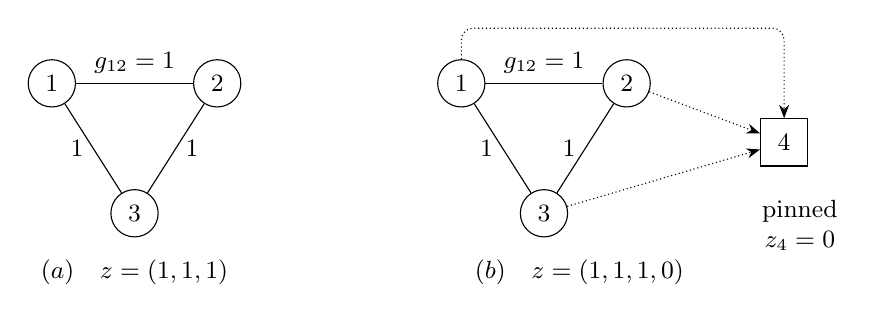
\begin{tikzpicture}[x=1cm,y=1cm,vertex/.style={circle,draw,minimum size=6mm,inner sep=1pt},pin/.style={rectangle,draw,minimum size=6mm,inner sep=1pt},every node/.style={font=\small}]
\node[vertex] (a1) at (0,1.2) {$1$};
\node[vertex] (a2) at (2.1,1.2) {$2$};
\node[vertex] (a3) at (1.05,-.45) {$3$};
\draw (a1)--node[above] {$g_{12}=1$}(a2);
\draw (a1)--node[left] {$1$}(a3);
\draw (a2)--node[right] {$1$}(a3);
\node at (1.05,-1.2) {$(a)\quad z=(1,1,1)$};
\node[vertex] (b1) at (5.2,1.2) {$1$};
\node[vertex] (b2) at (7.3,1.2) {$2$};
\node[vertex] (b3) at (6.25,-.45) {$3$};
\node[pin] (b4) at (9.3,.45) {$4$};
\draw (b1)--node[above] {$g_{12}=1$}(b2);
\draw (b1)--node[left] {$1$}(b3);
\draw (b2)--node[left] {$1$}(b3);
\draw[densely dotted,-{Stealth[length=1.7mm]}] (b2)--(b4);
\draw[densely dotted,-{Stealth[length=1.7mm]}] (b3)--(b4);
\draw[densely dotted,rounded corners=1.5mm,-{Stealth[length=1.7mm]}] (b1.north) -- (5.2,1.9) -- (9.3,1.9) -- (b4.north);
\node[align=center] at (9.5,-.6) {pinned\\$z_4=0$};
\node at (6.7,-1.2) {$(b)\quad z=(1,1,1,0)$};
\end{tikzpicture}

\caption{Two ambiguity structures. On the left, a balanced three-coordinate component has one direction supported on all three vertices, so its distance is three. On the right, an anchor is pinned by one-sided pair entries while the original three-coordinate component stays free. This is the distance-three construction in dimension four. Solid edges carry nonzero reciprocal gains; dotted arrows represent pinning information, not equality constraints. The graph describes diagonal changes, not causal relationships.}\label{fig:components}
\end{figure}


\subsection{Generic uniqueness and the low-dimensional boundary}
The graph also separates structured nonuniqueness from typical parameter choices.  The following statement concerns the parameterized odeco model, not an arbitrary distribution on mixed observations.

\begin{theorem}[Dimension threshold for generic mixed identifiability]\label{thm:generic-rigidity}
Let $1\le r\le n$, let $U=[u_1\ \cdots\ u_r]$ have Haar distribution on the Stiefel manifold, and let $\lambda\in\R^r$ be independent of $U$ with a distribution absolutely continuous with respect to Lebesgue measure.  Form
\[
 T=\sum_{a=1}^r\lambda_a u_a^{\otimes3}
\]
and let $H$ be its mixed part.  If $n\le2$, every nonempty fiber $\calF(H)$ has positive dimension.  If $n\ge3$, then
\[
 \Pr\{\calF(H)=\{(T_{111},\ldots,T_{nnn})\}\}=1.
\]
\end{theorem}
\begin{proof}
For $n=1$, $L_H$ has no rows.  For $n=2$, there is only one slice-pair diagonal equation, so $\rank L_H\le1<n$; a consistent fiber cannot be a singleton.

Now let $n\ge3$.  Fix $i<j<k$.  Almost surely the first Haar column has no zero coordinate, hence the coefficient vector
$((u_a)_i(u_a)_j(u_a)_k)_{a=1}^r$ is nonzero.  Conditional on such a $U$, the equation
$T_{ijk}=0$ is one proper hyperplane in $\lambda$ and therefore has probability zero.  A finite union over triples shows that every all-distinct entry is nonzero almost surely.  Every vertex belongs to at least one triple, so~\eqref{eq:triple-kernel} pins every coordinate of $\ker L_H$ to zero.  The diagonal of $T$ supplies consistency; hence the fiber is the asserted singleton.
\end{proof}

Thus the Cauchy components classified below form exceptional algebraic geometry rather than a generic failure mode.  They remain essential: the theorem is almost-sure, whereas the exact certificate must handle every observation, including those exceptional fibers and inconsistent arrays.

\subsection{Uniform identifiability under a support family}
For a nonempty fiber, define its diagonal distance by
\begin{equation}\label{eq:distance}
 d(H)=\min\{\norm{z}_0:0\ne z\in\ker L_H\},
 \qquad \norm{z}_0=|\supp z|,
\end{equation}
with $d(H)=\infty$ when the kernel is zero. Theorem~\ref{thm:graph} gives $d(H)=\min_{C\in\calC(H)}|C|$. This minimum is over actual tensor ambiguities, not only a linearized model.

\begin{theorem}[Exact support criterion]\label{thm:correction}
Suppose $\calF(H)\ne\varnothing$ and let $\calS$ be a nonempty family of allowed support sets. The clean completion in~\eqref{eq:exact-model} is unique for every $x^*\in\calF(H)$ and every allowed error if and only if
\begin{equation}\label{eq:support-condition}
 C\not\subseteq S\cup S'
 \quad\text{for every }C\in\calC(H)\text{ and }S,S'\in\calS.
\end{equation}
For at most $s$ unknown errors this is equivalent to $d(H)>2s$. For known erasures in a set $S$, it is equivalent to no free component being contained in $S$.
\end{theorem}
\begin{proof}
If two explanations yield the same observation, write $d=x+e=x'+e'$ with $x,x'\in\calF(H)$. Then $z=x'-x=e-e'$ belongs to $\ker L_H$ and is supported in $S\cup S'$ for allowed supports $S,S'$. If $z\ne0$, its support contains an entire free component by~\eqref{eq:graph-null}, contradicting~\eqref{eq:support-condition}.

Conversely, let a free component $C$ lie in $S\cup S'$ and choose a nonzero direction $z$ supported on $C$. Split $C$ into disjoint sets $A\subseteq S$ and $B\subseteq S'$. Put $e=z$ on $A$ and zero elsewhere, and put $e'=-z$ on $B$ and zero elsewhere. Then $e-e'=z$. For any $x\in\calF(H)$, both $x$ and $x'=x+z$ are completions and satisfy $x+e=x'+e'$. Thus uniform uniqueness fails.

A set of size at most $2s$ can be partitioned into two sets of size at most $s$, and no union of two such sets has more than $2s$ elements. This proves the cardinality criterion. For known erasures, two completions are indistinguishable precisely when their difference is supported in $S$, which proves the last claim.
\end{proof}

The distinction between known and unknown supports costs a factor of two because the two competing explanations may use different supports. The theorem also covers $s=0$, $n=1$, and a zero-dimensional fiber. When $d(H)=\infty$, mixed entries alone determine the tensor and any number of diagonal entries may be corrupted.

\begin{corollary}[Full-rank ambiguities persist]\label{cor:fullrank}
If a fiber contains a full-rank tensor and condition~\eqref{eq:support-condition} fails, uniform identifiability also fails when competing tensors are restricted to full rank.
\end{corollary}
\begin{proof}
Let $x$ represent a full-rank completion and let $z$ be the ambiguity direction used in the converse proof. A nonzero $n\times n$ unfolding minor remains nonzero for all sufficiently small perturbations $x+\tau z$. Take $\tau\ne0$ in that neighborhood. Both tensors are odeco by Theorem~\ref{thm:affine}, so their unfolding rank equals their tensor rank by Lemma~\ref{lem:unique-factors}. Splitting $\tau z$ into the two errors gives the same indistinguishability construction.
\end{proof}

\subsection{Pointwise decoding and finite or infinite lists}
Uniform correction is a worst-case statement. For a particular reported diagonal $d$, useful recovery may be possible even when the worst-case distance condition fails. Fix a particular solution $x^0$ and the basis $z_C$. Coordinates outside the union of free components are rigid. Let
\begin{align}
 b&=\big|\{i\notin\bigcup_C C:d_i\ne x^0_i\}\big|,\label{eq:rigid-errors}\\
 \rho_i&=(d_i-x^0_i)/(z_C)_i\quad(i\in C),\label{eq:ratios}\\
 \nu_C(\rho)&=|\{i\in C:\rho_i=\rho\}|,\qquad
 M_C=\max_\rho\nu_C(\rho).\label{eq:frequency}
\end{align}
The denominator in~\eqref{eq:ratios} is never zero. An arbitrary completion has the form $x^0+\sum_C\alpha_Cz_C$. Its disagreement count with $d$ is
\begin{equation}\label{eq:disagreement}
 b+\sum_C\big(|C|-\nu_C(\alpha_C)\big),
\end{equation}
where $\nu_C(\alpha)=0$ for an unobserved ratio.

\begin{theorem}[Pointwise list formula]\label{thm:list}
Let $\calF(H)\ne\varnothing$. The minimum number of diagonal changes needed to reach a completion is
\begin{equation}\label{eq:minimum-errors}
 m_0=b+\sum_C(|C|-M_C).
\end{equation}
The minimizing completions are obtained by choosing a modal ratio independently on each free component. Their number is the product of the numbers of distinct modal ratios.

If there is at least one free component, the list of completions within $s$ changes is infinite exactly when
\begin{equation}\label{eq:infinite-threshold}
 s\ge m_0+\min_C M_C.
\end{equation}
Below this threshold, its size is zero for $s<m_0$ and otherwise equals the sum of coefficients of degrees at most $s-m_0$ in
\begin{equation}\label{eq:list-polynomial}
 \prod_{C\in\calC(H)}
 \left(\sum_{\rho:\nu_C(\rho)>0}q^{M_C-\nu_C(\rho)}\right).
\end{equation}
If there are no free components, the list contains the single completion exactly when $s\ge b$.
\end{theorem}
\begin{proof}
Formula~\eqref{eq:disagreement} is separable in the component parameters. Minimizing each term maximizes its frequency, proving~\eqref{eq:minimum-errors} and the modal count. An unobserved value of $\alpha_C$ costs $|C|$ errors on component $C$, which is $M_C$ more than its minimum. There are infinitely many unobserved real values. Choosing modal values on the other components proves sufficiency of~\eqref{eq:infinite-threshold}.

Conversely, below that threshold no component parameter can be unobserved, since this alone costs at least $m_0+M_C$ errors. Each parameter is then drawn from a finite set. A choice of an observed ratio contributes excess cost $M_C-\nu_C(\rho)$. Multiplying the generating polynomials counts every tuple of choices with its total excess cost. Distinct tuples give distinct completions because the component directions are independent. This proves the finite count and also the necessity of the infinity criterion. With no free components there is only $x^0$.
\end{proof}

The formulas are invariant to rescaling a direction or changing the particular solution: these operations merely apply an invertible affine change to the ratios on each component. Exact equality of ratios is appropriate to the noiseless model. It is not a tolerance rule for sampled moments; bounded perturbations require a separate argument.

A useful baseline distinction is between counts and coordinate-weighted fitting. On a component with $z=(100,1,1)$ and ratios $(2,1,1)$, the modal parameter is $1$. Ordinary absolute diagonal residuals minimize
\[
 100|\alpha-2|+|\alpha-1|+|\alpha-1|,
\]
whose minimizer is $2$. Normalizing each residual by $|z_i|$ restores the unweighted median. This example isolates the effect of direction scaling; it is not evidence of a performance advantage over a general robust tensor method.

\section{Which ambiguity components can occur?}\label{sec:cauchy}
The graph theorem describes the kernel of a linear map for any mixed tensor. It does not yet use consistency. This section shows that a nonempty completion fiber imposes a much stronger internal geometry on each free component. The result also supplies explicit tensors on which the correction threshold is sharp.

\subsection{Associativity forces a clique}
\begin{lemma}[Internal closure]\label{lem:clique}
Suppose $\calF(H)\ne\varnothing$. Every free component $C$ is a clique. Moreover, every all-distinct entry involving a vertex of $C$ vanishes.
\end{lemma}
\begin{proof}
A nonzero all-distinct entry pins its three vertices. A free vertex belongs to no such entry, proving the second assertion.

Choose a completion $T$ and use its associative product from Lemma~\ref{lem:commuting}. For distinct $i,j\in C$, all terms with a third different index vanish, so
\begin{equation}\label{eq:two-product}
 e_i*e_j=a_{ij}e_i+a_{ji}e_j.
\end{equation}
For three distinct vertices $i,j,k\in C$, equate the $e_i$ coefficients in $(e_i*e_j)*e_k=e_i*(e_j*e_k)$. This gives
\begin{equation}\label{eq:associativity-clique}
 a_{ij}a_{ik}=a_{ij}a_{jk}+a_{ik}a_{kj}.
\end{equation}
If $i,j$ and $j,k$ are edges, then $a_{ij}a_{jk}\ne0$. Were $a_{ik}=0$, equation~\eqref{eq:associativity-clique} would give a contradiction. The kernel relation on a free component has nonzero coordinates, so $a_{ik}\ne0$ also implies $a_{ki}\ne0$. Thus every two-edge path is completed by an edge. Repeatedly shortening a path shows that any two vertices in a connected free component are adjacent.
\end{proof}

The restriction to a consistent fiber is necessary. Balanced graphs with a non-clique component can be formed algebraically from chosen pair entries, but their constant commutator equations have no solution. A kernel calculation alone would incorrectly regard such a graph as a realizable tensor ambiguity.

\begin{theorem}[Cauchy form of a free component]\label{thm:cauchy-form}
Suppose $\calF(H)\ne\varnothing$ and let $C$ be a free component with at least two vertices. Choose any kernel direction $z$ supported exactly on $C$. There are pairwise distinct real numbers $(t_i)_{i\in C}$ such that
\begin{equation}\label{eq:cauchy-form}
 a_{ij}=\frac{1}{z_j(t_j-t_i)}\qquad(i,j\in C,\ i\ne j).
\end{equation}
For fixed $z$, the nodes are determined up to a common translation. Rescaling $z$ by $c\ne0$ rescales all node differences by $c^{-1}$.
\end{theorem}
\begin{proof}
All $a_{ij}$ inside $C$ are nonzero by Lemma~\ref{lem:clique}. The pair kernel equations imply
\begin{equation}\label{eq:reverse-pair}
 a_{ji}=-\frac{z_j}{z_i}a_{ij}.
\end{equation}
Define $d_{ij}=1/(z_ja_{ij})$. Equation~\eqref{eq:reverse-pair} gives $d_{ji}=-d_{ij}$. Substituting $a_{kj}=-(z_k/z_j)a_{jk}$ into~\eqref{eq:associativity-clique}, dividing by the nonzero product $a_{ij}a_{ik}a_{jk}$, and then by $z_k$ gives
\[
 \frac{1}{z_ka_{jk}}=\frac{1}{z_ka_{ik}}-\frac{1}{z_ja_{ij}}.
\]
Equivalently,
\begin{equation}\label{eq:cocycle}
 d_{ik}=d_{ij}+d_{jk}.
\end{equation}
Fix a root $o\in C$, set $t_o=0$, and set $t_i=d_{oi}$ for $i\ne o$. Antisymmetry and~\eqref{eq:cocycle} imply $d_{ij}=t_j-t_i$. For a two-vertex component the same construction works without a triple equation. Since every $d_{ij}$ is nonzero, the nodes are pairwise distinct. Equation~\eqref{eq:cauchy-form} and the gauge statements now follow directly.
\end{proof}

The theorem concerns the \emph{internal mixed entries} of a free component. It does not say that its coordinates form an isolated direct summand of the tensor. For $i\in C$ and $j\notin C$, an entry $a_{ij}\ne0$ with $a_{ji}=0$ is possible: it pins $j$ but not $i$. Such couplings are important in the full-rank construction below. Discarding them would lead to a false block-decomposition claim.

The use of ``Cauchy'' in~\eqref{eq:cauchy-form} refers to reciprocal node differences with a column scaling. It does not assert that the full tensor is a classical symmetric Cauchy tensor with entries obtained by reciprocal sums of generating coordinates. The zeros on all-distinct entries and the freely varying diagonal are part of the construction.

\subsection{An explicit spectral realization}
We now prove that the internal form is realizable for any number of vertices. This supplies more than a consistency argument: the nonzero orthogonal components have an explicit description through one-variable roots.

\begin{theorem}[Spectral Cauchy family]\label{thm:spectral}
Let $m\ge1$, let $t_1,\ldots,t_m$ be distinct real numbers, and let $z_1,\ldots,z_m$ be nonzero. Put
\begin{equation}\label{eq:cauchy-defs}
 w_i=z_i^{-2},\qquad
 f_i=\sum_{j\ne i}\frac{w_j}{t_j-t_i}.
\end{equation}
For $\kappa\in\R$, define a symmetric cubic tensor $T(\kappa)$ by
\begin{align}
 T_{iii}(\kappa)&=z_i(\kappa-f_i),\label{eq:cauchy-diagonal}\\
 T_{iij}(\kappa)&=\frac{1}{z_j(t_j-t_i)}\quad(i\ne j),\label{eq:cauchy-pairs}\\
 T_{ijk}(\kappa)&=0\quad(i,j,k\text{ all distinct}).\nonumber
\end{align}
Every $T(\kappa)$ is real orthogonally decomposable. Its rank is $m$ if $\kappa\ne0$ and $m-1$ if $\kappa=0$. Its mixed part has fiber
\begin{equation}\label{eq:cauchy-fiber}
 \calF(P_{\rm mix}T)=x(0)+\spanof\{z\},
\end{equation}
and distance $m$.

More explicitly, let $g(\rho)=\sum_i w_i/(t_i-\rho)$. For every real root $\rho$ of $g(\rho)=\kappa$, define
\begin{equation}\label{eq:cauchy-eigen}
 r_i(\rho)=\frac{1}{z_i(t_i-\rho)},\qquad
 \lambda(\rho)=\sqrt{g'(\rho)},\qquad
 u(\rho)=\frac{r(\rho)}{\lambda(\rho)}.
\end{equation}
Then
\begin{equation}\label{eq:cauchy-decomposition}
 T(\kappa)=\sum_{\rho:g(\rho)=\kappa}\lambda(\rho)u(\rho)^{\otimes3}.
\end{equation}
For $\kappa=0$, the common nullspace has the additional direction $(1/z_i)_{i=1}^m$.
\end{theorem}
\begin{proof}
Relabel so $t_1<\cdots<t_m$. On every open interval between successive nodes,
\[
 g'(\rho)=\sum_i\frac{w_i}{(t_i-\rho)^2}>0,
\]
and $g$ increases from $-\infty$ to $+\infty$. There is one simple root of $g(\rho)=\kappa$ in each such interval. To the left of $t_1$, $g$ increases from $0$ to $+\infty$, giving one additional root precisely when $\kappa>0$. To the right of $t_m$, it increases from $-\infty$ to $0$, giving one precisely when $\kappa<0$. Therefore there are $m$ roots for nonzero $\kappa$ and $m-1$ for zero $\kappa$. No root equals a node.

For any root $\rho$, $\norm{r(\rho)}^2=g'(\rho)$, so $u(\rho)$ is a unit vector. If $\rho\ne\sigma$ are two roots, then
\begin{equation}\label{eq:root-orthogonality}
 \ip{r(\rho)}{r(\sigma)}
 =\sum_i\frac{w_i}{(t_i-\rho)(t_i-\sigma)}
 =\frac{g(\rho)-g(\sigma)}{\rho-\sigma}=0.
\end{equation}
Thus the root vectors are mutually orthogonal.

It remains to verify that these vectors diagonalize the slices with exactly the coefficients in~\eqref{eq:cauchy-decomposition}. Fix a root $\rho$ and write $r=r(\rho)$. For $j\ne i$, the only nonzero terms in row $j$ of slice $T_i$ are in columns $i,j$, so
\begin{align*}
 (T_ir)_j
 &=\frac{r_i}{z_j(t_j-t_i)}
    -\frac{r_j}{z_i(t_j-t_i)}\\
 &=\frac{1}{z_iz_j(t_j-t_i)}
   \left(\frac{1}{t_i-\rho}-\frac{1}{t_j-\rho}\right)
 =r_ir_j.
\end{align*}
For row $i$, equations~\eqref{eq:cauchy-defs}--\eqref{eq:cauchy-pairs} give
\begin{align*}
 (T_ir)_i
 &=\frac{\kappa-f_i}{t_i-\rho}
   +\sum_{j\ne i}\frac{w_j}{(t_j-t_i)(t_j-\rho)}\\
 &=\frac{1}{t_i-\rho}
   \left(\kappa-\sum_{j\ne i}\frac{w_j}{t_j-\rho}\right)
 =\frac{w_i}{(t_i-\rho)^2}=r_i^2.
\end{align*}
The penultimate equality uses $g(\rho)=\kappa$. Hence $T_ir=r_ir$, or
\begin{equation}\label{eq:slice-eigen}
 T_iu=\lambda(\rho)u_i u.
\end{equation}
When $\kappa\ne0$, these are $m$ orthonormal vectors, a complete basis. Equality~\eqref{eq:slice-eigen} proves~\eqref{eq:cauchy-decomposition} slice by slice.

When $\kappa=0$, let $v_i=1/z_i$. Direct substitution shows $(T_iv)_j=0$ for $j\ne i$, since its two terms cancel. In row $i$ the diagonal term is $-f_i$ and the off-diagonal sum is $f_i$, so $T_iv=0$. Moreover,
\[
 \ip{v}{r(\rho)}=\sum_i\frac{w_i}{t_i-\rho}=g(\rho)=0.
\]
The $m-1$ root vectors together with $v/\norm v$ are an orthonormal basis. All $\lambda(\rho)$ are positive, giving the decomposition and the asserted ranks by Lemma~\ref{lem:unique-factors}. This reasoning also covers $m=1$: there is one root for nonzero $\kappa$, and the zero tensor for $\kappa=0$.

Finally, all pair entries are nonzero and satisfy $a_{ji}z_i+a_{ij}z_j=0$, while every all-distinct entry is zero. The graph is a single balanced free clique. Theorem~\ref{thm:graph} gives a one-dimensional kernel supported on all $m$ vertices, and Theorem~\ref{thm:affine} yields~\eqref{eq:cauchy-fiber}. Its distance is $m$.
\end{proof}

The theorem proves that a one-dimensional fiber can have any support size. Varying $\kappa$ changes the tensor only on the diagonal, but its orthogonal factors move through the roots of a secular equation. The ambiguity is consequently not merely a relabeling of fixed factors. A rank drop occurs at $\kappa=0$; everywhere else the family has full rank.

\subsection{A three-coordinate example}
Take $m=3$, $z=(1,1,1)$, and $t=(0,1,1/2)$. Then $f=(3,-3,0)$ and
\[
 x(\kappa)=(\kappa-3,\kappa+3,\kappa).
\]
The mixed entries are
\begin{equation}\label{eq:three-example}
 a_{12}=1,\ a_{21}=-1,\ a_{13}=2,\ a_{31}=-2,
 \ a_{23}=-2,\ a_{32}=2,\qquad h_{123}=0.
\end{equation}
Every edge gain is one. The fiber is a line with direction $(1,1,1)$, so $d(H)=3$. No one- or two-coordinate ambiguity exists. The tensor at $\kappa=0$ has rank two, and every nonzero $\kappa$ has rank three.

This example is small enough to expose an important testing boundary. An enumeration in which each mixed orbit belongs only to $\{-1,0,1\}$ cannot contain it. An apparent absence of three-coordinate ambiguities in that enumeration is not a proof that they never occur. Enlarging the pair alphabet to include $\pm2$ produces the example exactly. Its role is to falsify a structural conjecture, not to estimate the frequency of ambiguities under a distribution of latent models.

For a reported diagonal $d=(-2,4,2)$, the ratios relative to $x(0)=(-3,3,0)$ are $(1,1,2)$. The modal completion has $\kappa=1$ and requires one change. At budget two, the completion $\kappa=2$ is also possible. At budget three, every unobserved parameter value is admissible, so the list becomes infinite. This illustrates the difference between unique nearest completion, uniform one-error correction, and a budget-dependent list.

\subsection{Every distance at full tensor rank}
A direct sum of a distance-$m$ family with a purely diagonal tensor does not realize distance $m$ in a larger ambient space: the added isolated coordinates create distance-one ambiguities. A coupling is needed to make the complement rigid without pinning the desired free component.

\begin{theorem}[Full-rank distance spectrum]\label{thm:all-distances}
For every $n\ge1$ and every integer $1\le m\le n$, there is a rational tensor $T\in\odeco$ of rank $n$ whose mixed part has a one-dimensional fiber and distance exactly $m$.
\end{theorem}
\begin{proof}
For $m=n$, use Theorem~\ref{thm:spectral} with $t_i=i-1$, $z_i=1$, and $\kappa=1$. Suppose $m<n$. Begin with the same $m$-coordinate Cauchy tensor and add an anchor coordinate $q=m+1$. Modify the original diagonal by subtracting $t_i$, and set
\begin{equation}\label{eq:anchor}
 T_{iiq}=1\quad(i\le m),\qquad T_{iqq}=0\quad(i\le m),\qquad
 T_{qqq}=1,
\end{equation}
with symmetry understood and all other new mixed entries zero. The anchor slice on these $m+1$ coordinates is the identity.

We verify that the augmented slices commute. The original Cauchy slices commute. Changing their diagonal entries by $-t_i$ affects the $(i,j)$ commutator entry, for $i\ne j\le m$, by
\[
 -t_i a_{ji}-t_j a_{ij}
 =(t_i-t_j)\frac{1}{t_j-t_i}=-1.
\]
The new anchor products contribute $+1$ at that entry, canceling the change. Other entries within the original block are unchanged because all distinct-index coefficients vanish. At an entry $(i,q)$ of the commutator for slices $i,j$, the two terms are $T_{iij}$ and $T_{jii}$, which are equal by symmetry, so they cancel. The $(j,q)$ entry cancels in the same way, and all remaining anchor entries are zero. The anchor slice commutes because it is the identity. Lemma~\ref{lem:commuting} proves that this block is odeco. Its identity slice has rank $m+1$, so the block's tensor rank is $m+1$.

If $n>m+1$, take a direct sum with nonzero rational diagonal components on the remaining coordinates. The resulting tensor is odeco and has rank $n$. It still has unwanted isolated ambiguities, which the following rotation removes.

Let $k=n-m$ be the size of the complement, including the anchor. On that complement use the rational orthogonal Householder matrix
\begin{equation}\label{eq:householder}
 R=I-\frac{2vv^\top}{v^\top v},\qquad v=(1,2,\ldots,k)^\top,
\end{equation}
and act as the identity on the first $m$ coordinates. Every entry of the first column of $R$ is nonzero. For $k=1$ it is $-1$; for $k\ge2$, its first entry is $1-2/\sum_{j=1}^k j^2>0$, and the others are $-2j/\sum_{j=1}^k j^2$.

After this orthogonal change of basis, the internal Cauchy entries on the first $m$ coordinates are unchanged. For $i\le m$ and every complementary coordinate $j$, the new entries satisfy
\[
 T_{iij}=R_{j,q}\ne0,\qquad T_{ijj}=0.
\]
Every complementary vertex is therefore pinned by a one-sided pair. All-distinct entries involving an original vertex remain zero: before rotation there were no entries with that vertex and two complementary indices, nor with two different original vertices and a complementary index. The first $m$ vertices retain their single balanced clique and are unpinned. The graph has exactly one free component of size $m$. Orthogonal rotation preserves tensor rank and orthogonal decomposability, and every coefficient is rational. Theorems~\ref{thm:affine} and~\ref{thm:graph} complete the proof.
\end{proof}

\subsection{What rank and incoherence do not determine}
The full-rank spectrum shows that rank alone cannot determine the correction distance. Even maximally flat orthogonal factors do not guarantee one-error correction. In dimension two, take
\[
 U=\frac{1}{\sqrt2}\begin{pmatrix}1&1\\1&-1\end{pmatrix},
 \qquad (\lambda_1,\lambda_2)=(2\sqrt2,4\sqrt2).
\]
The symmetric orbits $(T_{111},T_{112},T_{122},T_{222})$ are $(3,-1,3,-1)$. The tensor has rank two and the flatness parameter $\sqrt n\max_{ia}|u_{ia}|$ equals one. Its mixed graph is one free pair, so $d(H)=2$ and uniform correction of one error is impossible. This does not refute incoherence-based robust recovery theorems, whose additional rank and sparsity conditions must also hold. It shows why flatness alone is not a certificate for the current mask.

A fixed lower rank can alter a fiber in the opposite direction. For $n=2$ and nonzero mixed entries $a=T_{112}$, $b=T_{122}$, a rank-one symmetric tensor must have
\begin{equation}\label{eq:rank-one}
 T_{111}=\frac{a^2}{b},\qquad T_{222}=\frac{b^2}{a}.
\end{equation}
Indeed, for $T=\lambda u^{\otimes3}$ the first ratio is $\lambda u_1^3$ and the second is $\lambda u_2^3$. Conversely, these values make all the entries a rank-one cubic, by taking the ratio $u_2/u_1=b/a$ and normalizing. The unrestricted odeco fiber is a line, whereas its rank-one part is a point. Our exact distance is therefore stated for the union of ranks, with Corollary~\ref{cor:fullrank} covering full-rank competition, not for every separately fixed lower rank.

\section{A posterior certificate with bounded mixed noise}\label{sec:stability}
Exact equality of measured mixed entries is a strong assumption. We now allow a bounded perturbation in those entries and a bounded error on the otherwise clean diagonal coordinates. Gross diagonal errors still have no amplitude bound. The certificate is conditional: it bounds every true tensor satisfying a declared observation model, but does not establish that such a tensor exists.

\subsection{Observation uncertainty and a restricted margin}
Suppose the observed mixed tensor is $\widehat H$, and the reported diagonal is $d$. A compatible truth satisfies
\begin{align}
 T^*&=H^*+D(x^*)\in\odeco,\qquad
 \widehat H=H^*+E,\quad P_{\rm mix}E=E,\quad \norm E_F\le\delta,\label{eq:noisy-mixed}\\
 d&=x^*+e+v,\qquad |\supp e|\le s,\quad \norm v\le\epsilon.\label{eq:noisy-diag}
\end{align}
The numbers $\delta,\epsilon\ge0$ are supplied deterministic bounds. They are not estimated confidence levels. The perturbation $E$ is symmetric because both mixed tensors are symmetric.

Let an arbitrary candidate procedure return $\widehat x\in\R^n$ and a candidate gross-error support $\widehat S$ with $|\widehat S|\le s$. The theorem below does not require that this procedure minimize an objective. Write
\begin{equation}\label{eq:noisy-residuals}
 r=\norm{L_{\widehat H}\widehat x+c_{\widehat H}},
 \qquad e_0=\norm{P_{\widehat S^c}(d-\widehat x)}.
\end{equation}
Here $P_A$ restricts a vector to coordinates in $A$. Define the restricted margin
\begin{equation}\label{eq:beta}
 \beta=\min_{S\subseteq[n],\ |S|\le s}
 \sigma_{\min}\!\begin{pmatrix}
 L_{\widehat H}\\ P_{(S\cup\widehat S)^c}
 \end{pmatrix}.
\end{equation}
The minimum includes every possible true gross-error support. Its second block retains only coordinates clean under both the true and candidate explanations. This is why a support union, rather than the candidate support alone, appears in the certificate.

A singular mixed-only operator need not make $\beta$ zero. On a distance-three fiber with $s=1$, any union of two allowed singleton supports leaves a clean coordinate on the free component. That coordinate fixes its free parameter. Conversely, if a free component fits inside such a union, the corresponding restricted operator has a nonzero kernel and no positive margin is possible in the exact model.

\subsection{Perturbing the completion equations}
\begin{lemma}[Perturbing the coefficients]\label{lem:perturbation}
For mixed symmetric cubics $A,E$,
\begin{align}
 \norm{L_E}_{2\to2}&\le\norm E_F,\label{eq:l-perturb}\\
 \norm{c_{A+E}-c_A}&\le2\norm A_F\norm E_F+\norm E_F^2.\label{eq:c-perturb}
\end{align}
\end{lemma}
\begin{proof}
Apply the energy identity to $E$. For each pair,
\[
 (E_{ijj}z_i+E_{iij}z_j)^2
 \le(E_{ijj}^2+E_{iij}^2)(z_i^2+z_j^2)
 \le(E_{ijj}^2+E_{iij}^2)\norm z^2.
\]
For each triple, its term is at most $2E_{ijk}^2\norm z^2$. The full Frobenius norm of $E$ counts each pair orbit three times and each all-distinct orbit six times. Summing proves~\eqref{eq:l-perturb}, with a deliberately conservative constant.

For the second inequality, retain all ordered slice pairs and all matrix entries temporarily. A family of skew matrices $B_{ij}$ with $B_{ji}=-B_{ij}$ has full squared norm four times the squared norm of its entries with $i<j,p<q$. Thus restriction to our independent entries divides its norm by two. The bilinear family $[A_i,E_j]$ has norm at most $2\norm A_F\norm E_F$, since
\[
 \sum_{i,j}\norm{[A_i,E_j]}_F^2
 \le4\sum_{i,j}\norm{A_i}_F^2\norm{E_j}_F^2.
\]
The cross family $[A_i,E_j]+[E_i,A_j]$ therefore has full norm at most $4\norm A_F\norm E_F$, by the triangle inequality. It has the required skew symmetries, so its restricted norm is at most $2\norm A_F\norm E_F$. The family $[E_i,E_j]$ similarly has restricted norm at most $\norm E_F^2$. Expanding the commutator of $A+E$ gives~\eqref{eq:c-perturb}.
\end{proof}

The constants use the full tensor Frobenius norm. A norm on a list of distinct symmetric orbits without their multiplicities would not satisfy the same statement without adjustment. The implementation expands the symmetric array when calculating these norms.

\begin{theorem}[Conditional posterior radius]\label{thm:posterior}
Assume~\eqref{eq:noisy-mixed}--\eqref{eq:noisy-diag}. Let $\gamma$ be any certified lower bound on $\beta$ in~\eqref{eq:beta}, with $\gamma>\delta$. Define
\begin{equation}\label{eq:ab}
 A=r+\delta(\norm{\widehat x}+2\norm{\widehat H}_F)+\delta^2,
 \qquad B=e_0+\epsilon.
\end{equation}
Then every compatible truth satisfies
\begin{equation}\label{eq:posterior}
 \norm{\widehat x-x^*}\le
 R:=\frac{\sqrt{A^2+B^2}}{\gamma-\delta},
 \qquad
 \norm{\widehat H+D(\widehat x)-T^*}_F
 \le\sqrt{\delta^2+R^2}.
\end{equation}
No bound on $\norm e$ is required.
\end{theorem}
\begin{proof}
Let $S^*=\supp e$ and $w=\widehat x-x^*$. Since $x^*$ is a completion of $H^*$, its exact residual is zero. Linearity of $L_H$ in $H$ and Lemma~\ref{lem:perturbation}, applied with $A=\widehat H$ and perturbation $-E$, give
\begin{align*}
 \norm{L_{\widehat H}x^*+c_{\widehat H}}
 &\le\norm{L_E x^*}+\norm{c_{\widehat H}-c_{H^*}}\\
 &\le\delta\norm{x^*}+2\delta\norm{\widehat H}_F+\delta^2.
\end{align*}
Subtracting the candidate residual yields
\[
 \norm{L_{\widehat H}w}
 \le r+\delta\norm{x^*}+2\delta\norm{\widehat H}_F+\delta^2
 \le A+\delta\norm w.
\]
On coordinates outside $S^*\cup\widehat S$, the gross error is absent and $d-x^*=v$. Therefore
\[
 \norm{P_{(S^*\cup\widehat S)^c}w}
 \le\norm{P_{\widehat S^c}(\widehat x-d)}+\norm v
 \le B.
\]
By the restricted margin, these two bounds imply
\[
 \gamma\norm w\le\sqrt{(A+\delta\norm w)^2+B^2}
 \le\sqrt{A^2+B^2}+\delta\norm w.
\]
The last step is the Euclidean triangle inequality in $\R^2$. Rearranging uses $\gamma>\delta$ and gives the first radius. The mixed and pure-diagonal tensor subspaces are orthogonal under the full Frobenius inner product, so the total squared error is $\norm E_F^2+\norm w^2$. This proves the second radius.
\end{proof}

The candidate tensor itself need not be odeco. A successful certificate bounds the distance from that candidate to every compatible odeco truth. It does not convert an approximately commuting tensor into an exactly commuting one. If two truths satisfy the same observation bounds, their tensor distance is at most twice the total radius by the triangle inequality. This is a deterministic identifiability-diameter statement, not a posterior probability distribution.

The proof uses no separation between component weights. It also gives no direct factor-error bound. Translating a tensor radius into stable individual factors requires additional quantitative hypotheses, especially near a rank drop. Those hypotheses should not be inferred from a successful diagonal certificate.

\subsection{Rational witnesses for the margin}
For rational observations, form the rational positive semidefinite matrices
\begin{equation}\label{eq:restricted-gram}
 M_S=L_{\widehat H}^\top L_{\widehat H}
       +\diag\big(\one_{i\notin S\cup\widehat S}\big)_{i=1}^n.
\end{equation}
A witness consists of a rational inverse $B_S$ for every $S$ with $|S|\le s$. The verifier checks $M_SB_S=I$ exactly. Since $M_S$ is already known to be positive semidefinite, invertibility makes it positive definite; its inverse has positive eigenvalues. Hence
\begin{equation}\label{eq:trace-bound}
 \lambda_{\min}(M_S)
 =\lambda_{\max}(M_S^{-1})^{-1}
 \ge\frac{1}{\tr(M_S^{-1})}.
\end{equation}
Any rational $\gamma>0$ satisfying
\begin{equation}\label{eq:gamma-cert}
 \gamma^2\tr(B_S)\le1\quad\text{for all }|S|\le s
\end{equation}
is a verified lower bound on $\beta$. The trace bound can be conservative, but its validity does not depend on a numerical eigensolver.

The remaining norms in~\eqref{eq:ab} can be bounded by rational upper values. For a nonnegative rational $a$, choose an integer $k$ so $(k/2^b)^2\le a<((k+1)/2^b)^2$ using integer square roots. The upper dyadic endpoint bounds $\sqrt a$; the lower endpoint can be used for a positive margin. With upper bounds $\bar r,\bar e_0,\bar n_x,\bar n_H$, the verifier checks nonnegativity, their squared inequalities, and
\begin{equation}\label{eq:radius-check}
 \bar R^2(\gamma-\delta)^2\ge
 [\bar r+\delta(\bar n_x+2\bar n_H)+\delta^2]^2
 +(\bar e_0+\epsilon)^2.
\end{equation}
Together with a squared total-radius check, these are exact rational comparisons. The unknown truth is not an input to this verifier.

Enumerating supports costs $\sum_{k=0}^s\binom nk$ inverse witnesses. This is not polynomial in unrestricted $s$. Our implementation explicitly caps that enumeration at 2,048 supports and the dimension at 16, while the theorem itself is not so bounded. For larger instances, a different certified lower bound on~\eqref{eq:beta} would be needed; silently omitting support sets would invalidate the certificate.


\subsection{A quantitative connection to the graph}
The graph decides whether a restricted margin is positive. It also separates two reasons why that margin can be small: weak control transverse to the fiber, and a retained coordinate with a small entry in its component direction. The following elementary bound makes this separation explicit. It is a conditioning consequence, not a replacement for checking consistency.

\begin{proposition}[A graph-based margin bound]\label{prop:graph-margin}
Suppose $0<\rank L_H<n$, and let $\tau$ be its smallest nonzero singular value. Let $A\subseteq[n]$ meet every free component and define
\begin{equation}\label{eq:alpha-margin}
 \alpha=\min_{C\in\calC(H)}
 \frac{\norm{P_Az_C}}{\norm{z_C}}>0.
\end{equation}
Then
\begin{equation}\label{eq:graph-margin}
 \sigma_{\min}\!\begin{pmatrix}L_H\\P_A\end{pmatrix}
 \ge \frac{\alpha\tau}{\sqrt{\tau^2+1+\alpha^2}}.
\end{equation}
If $\ker L_H=\{0\}$, the simpler lower bound $\sigma_{\min}(L_H)$ applies. If $L_H=0$, the stacked operator is nonsingular exactly when $A=[n]$, in which case its margin is one.
\end{proposition}
\begin{proof}
Write any vector as $v=p+q$, with $p\in\ker L_H$ and $q\perp\ker L_H$. Put $a=\norm{L_Hv}$ and $b=\norm{P_Av}$. The definition of $\tau$ gives $\norm q\le a/\tau$. Disjoint supports make the component directions orthogonal, before and after restriction. Hence $\norm{P_Ap}\ge\alpha\norm p$, so
\[
 \norm p\le \frac{b+\norm q}{\alpha}
 \le\frac{b}{\alpha}+\frac{a}{\alpha\tau}.
\]
Orthogonality of $p,q$ and the Frobenius bound on a matrix's operator norm imply
\begin{align*}
 \norm v^2
 &\le\left(\frac{a}{\alpha\tau}+\frac{b}{\alpha}\right)^2
       +\frac{a^2}{\tau^2}\\
 &\le\left(\frac{1}{\alpha^2\tau^2}
           +\frac{1}{\alpha^2}+\frac{1}{\tau^2}\right)(a^2+b^2).
\end{align*}
Rearrange and minimize over unit $v$ to obtain~\eqref{eq:graph-margin}. The two degenerate cases follow directly from the definition of the stacked operator.
\end{proof}

For the three-coordinate example, the nonzero eigenvalues of $G_H$ are six and twelve. Retaining a single coordinate gives $\alpha=1/\sqrt3$ and $\tau=\sqrt6$, hence the squared lower margin $3/11$. The direct inverse witnesses in Appendix~\ref{app:worked} give the slightly larger bound $24/85$. These are two independently justified lower bounds, not competing estimates of an unknown experimental quantity.

Component size alone does not control $\alpha$. A full-support direction can have one coordinate arbitrarily small relative to its norm. A retained coordinate at that position determines the component parameter exactly in the noiseless model, while providing weak Euclidean control under noise. Likewise, small mixed coefficients can reduce $\tau$ without changing any edge support. This explains why the exact threshold depends only on support containment but the posterior radius needs quantitative coefficients. For a support-union certificate, the bound must hold for every retained set, not only for a favorable one.

\subsection{Candidate generation and negative outcomes}
For the small validation instances, the candidate is obtained by exhaustively solving a least-squares problem for each possible discarded support:
\begin{equation}\label{eq:trimmed-ls}
 \min_{|S|\le s}\ \min_x
 \norm{L_{\widehat H}x+c_{\widehat H}}^2+\norm{P_{S^c}(d-x)}^2.
\end{equation}
Each nonsingular normal equation is solved with rational arithmetic. Singular cases are skipped by this candidate routine; the posterior verifier remains separate. The success of the certificate depends on its residual and margin, not on a claim that this exhaustive method scales well.

There are two informative ways to fail certification. A singular restricted matrix witnesses the absence of a positive margin for that support union. Even if every matrix is invertible, the conservative lower margin may not exceed the declared mixed-noise bound. Neither outcome proves that the observed tensor is incompatible with the model. Conversely, a small residual alone is not a substitute for either a positive margin or the existence assumption.

At zero mixed noise, the restricted margin recovers the exact obstruction. For a consistent $H$, a particular $M_S$ is singular precisely when there is a nonzero $z\in\ker L_H$ supported inside $S\cup\widehat S$. Theorem~\ref{thm:graph} makes this equivalent to containment of a free component. Thus the noisy theorem is anchored in the same support geometry as exact correction, rather than in a separate heuristic condition.

\begin{thebibliography}{99}
\bibitem[Anandkumar et~al.(2014)] {anandkumar2014}
Animashree Anandkumar, Rong Ge, Daniel Hsu, Sham M. Kakade, and Matus Telgarsky.
Tensor Decompositions for Learning Latent Variable Models.
\emph{Journal of Machine Learning Research}, 15(80):2773--2832, 2014.

\bibitem[Anandkumar et~al.(2016)] {anandkumar2016}
Anima Anandkumar, Prateek Jain, Yang Shi, and U. N. Niranjan.
Tensor vs. Matrix Methods: Robust Tensor Decomposition under Block Sparse Perturbations.
\emph{Proceedings of Machine Learning Research}, 51:268--276, 2016.

\bibitem[Ardiyansyah and Sodomaco(2023)] {ardiyansyah2023}
Muhammad Ardiyansyah, and Luca Sodomaco.
Dimensions of Higher Order Factor Analysis Models.
\emph{Algebraic Statistics}, 14(1):91--108, 2023.

\bibitem[Ashraphijuo and Wang(2017)] {ashraphijuo2017}
Morteza Ashraphijuo, and Xiaodong Wang.
Fundamental Conditions for Low-CP-Rank Tensor Completion.
\emph{Journal of Machine Learning Research}, 18(63):1--29, 2017.

\bibitem[Yuan(2026)] {yuan2026}
Ming Yuan.
On Spectral Learning for Odeco Tensors: Perturbation, Initialization, and Algorithms.
In \emph{Proceedings of the International Congress of Mathematicians 2026, Volume 7}, pages 463--482. Society for Industrial and Applied Mathematics, 2026.

\bibitem[Auddy and Yuan(2023)] {auddy2023}
Arnab Auddy and Ming Yuan.
Perturbation Bounds for (Nearly) Orthogonally Decomposable Tensors with Statistical Applications.
\emph{Information and Inference: A Journal of the IMA}, 12(2):1044--1072, 2023.

\bibitem[Bhaskara et~al.(2014)] {bhaskara2014}
Aditya Bhaskara, Moses Charikar, and Aravindan Vijayaraghavan.
Uniqueness of Tensor Decompositions with Applications to Polynomial Identifiability.
\emph{Proceedings of Machine Learning Research}, 35:742--778, 2014.

\bibitem[Boralevi et~al.(2017)] {boralevi2017}
Ada Boralevi, Jan Draisma, Emil Horobe\c{t}, and Elina Robeva.
Orthogonal and Unitary Tensor Decomposition from an Algebraic Perspective.
\emph{Israel Journal of Mathematics}, 222(1):223--260, 2017.

\bibitem[Haselby et~al.(2024)] {haselby2024}
Cullen Haselby, Mark Iwen, Santhosh Karnik, and Rongrong Wang.
Tensor Deli: Tensor Completion for Low CP-Rank Tensors via Random Sampling.
\emph{arXiv preprint arXiv:2403.09932}, 2024.

\bibitem[Kir\'aly et~al.(2015)] {kiraly2015}
Franz J. Kir\'aly, Louis Theran, and Ryota Tomioka.
The Algebraic Combinatorial Approach for Low-Rank Matrix Completion.
\emph{Journal of Machine Learning Research}, 16(41):1391--1436, 2015.

\bibitem[Koiran(2021)] {koiran2021}
Pascal Koiran.
Orthogonal Tensor Decomposition and Orbit Closures from a Linear Algebraic Perspective.
\emph{Linear and Multilinear Algebra}, 69(13):2353--2388, 2021.

\bibitem[Luo et~al.(2021)] {luo2021}
Yuetian Luo, Garvesh Raskutti, Ming Yuan, and Anru R. Zhang.
A Sharp Blockwise Tensor Perturbation Bound for Orthogonal Iteration.
\emph{Journal of Machine Learning Research}, 22(179):1--48, 2021.

\bibitem[Mickelin and Karaman(2023)] {mickelin2023}
Oscar Mickelin and Sertac Karaman.
Recovering Orthogonal Tensors under Arbitrarily Strong, but Locally Correlated, Noise.
\emph{Numerical Linear Algebra with Applications}, 30(4):e2479, 2023.

\bibitem[Robeva(2016)] {robeva2016}
Elina Robeva.
Orthogonal Decomposition of Symmetric Tensors.
\emph{SIAM Journal on Matrix Analysis and Applications}, 37(1):86--102, 2016.

\bibitem[Schramm and Weitz(2015)] {schramm2015}
Tselil Schramm, and Benjamin Weitz.
Symmetric Tensor Completion from Multilinear Entries and Learning Product Mixtures over the Hypercube.
\emph{arXiv preprint arXiv:1506.03137}, 2015.

\bibitem[Wu(2026)] {tongwu2026}
Tong Wu.
Guaranteed Nonconvex Low-Rank Tensor Estimation via Scaled Gradient Descent.
\emph{Journal of Machine Learning Research}, 27(9):1--90, 2026.

\bibitem[Xia and Zhou(2019)] {xia2019}
Dong Xia, and Fan Zhou.
The Sup-norm Perturbation of HOSVD and Low Rank Tensor Denoising.
\emph{Journal of Machine Learning Research}, 20(61):1--42, 2019.
\end{thebibliography}

\appendix
\section{Worked systems and boundary cases}\label{app:worked}
\subsection{The complete two-coordinate system}
A two-dimensional symmetric cubic is specified by four entries. Write
\[
 T_1=\begin{pmatrix}x_1&a\\a&b\end{pmatrix},\qquad
 T_2=\begin{pmatrix}a&b\\b&x_2\end{pmatrix}.
\]
There is one independent commutator equation,
\begin{equation}\label{eq:two-system}
 bx_1+ax_2=a^2+b^2.
\end{equation}
If $a=b=0$, every diagonal is a completion and the graph consists of two free singletons. If $a\ne0,b=0$, then $x_2=a$ while $x_1$ is free. The pair entry pins vertex two; it does not pin vertex one. If $a=0,b\ne0$, the roles reverse. If both are nonzero, the graph is one free pair and its direction can be chosen as $(a,-b)$.

These cases have distances one, one, one, and two, respectively. None has a unique mixed-only completion. Equation~\eqref{eq:two-system} is always consistent in dimension two, but this fact does not extend to dimension three. The point of the example is to verify the indexing and pin conventions before using a larger graph, not to extrapolate a universal low-dimensional obstruction.

For example, $a=-1,b=3$ gives $3x_1-x_2=10$, containing the full-rank tensor with diagonal $(3,-1)$. The nearby diagonal $(3+\tau,-1+3\tau)$ gives a different full-rank completion for all sufficiently small nonzero $\tau$. Its difference is supported on both coordinates. Splitting that difference across the two singleton supports produces an observation with two one-error explanations, exactly as in Theorem~\ref{thm:correction}.

\subsection{A fully explicit inconsistency witness}
Set all two-equal-index mixed entries of a three-dimensional tensor to zero, and set $H_{123}=1$. The mixed slices are
\[
 H_1=\begin{pmatrix}0&0&0\\0&0&1\\0&1&0\end{pmatrix},\quad
 H_2=\begin{pmatrix}0&0&1\\0&0&0\\1&0&0\end{pmatrix},\quad
 H_3=\begin{pmatrix}0&1&0\\1&0&0\\0&0&0\end{pmatrix}.
\]
The all-distinct entry pins all three vertices, and $L_H$ has full column rank. Nevertheless, the $(1,2)$ entry of $[H_1,H_2]$ is $-1$, while the corresponding row of $L_H$ is zero because its two coefficients are $H_{122}=H_{112}=0$. This single equation is $0=1$ in the right-side convention of~\eqref{eq:affine-main}. A unit vector on this row is a negative certificate. Thus even an all-pinned graph and full column rank do not establish existence.

This example is also a useful test of a verifier that checks only a candidate's diagonal equations but omits constant rows. A diagonal recovered from a selected square subsystem cannot satisfy the omitted $0=1$ equation. The complete direct-product check rejects it regardless of how accurately that square subsystem was solved.


\subsection{A complete three-coordinate positive certificate}
For the mixed entries in~\eqref{eq:three-example}, six of the nine independent commutator rows vanish identically. The remaining system is
\begin{equation}\label{eq:worked-matrix}
 \begin{pmatrix}-1&1&0\\-2&0&2\\0&2&-2\end{pmatrix}
 \begin{pmatrix}x_1\\x_2\\x_3\end{pmatrix}
 =\begin{pmatrix}6\\6\\6\end{pmatrix}.
\end{equation}
Its third row is twice its first row minus its second row, including the right side. Thus the apparent third constraint adds no rank and causes no inconsistency. A particular solution is $x^0=(-3,3,0)^\top$ and the vector $z=(1,1,1)^\top$ is a null direction. The first two rows and first two columns have determinant two. This minor proves rank at least two; the nonzero null vector proves rank at most two. These objects constitute the complete positive certificate. None of the six omitted rows may be dropped by an implementation without first checking that both its coefficient vector and its right side are zero.

The Gram matrix and two representative inverse witnesses are
\begin{align}
 G&=\begin{pmatrix}5&-1&-4\\-1&5&-4\\-4&-4&8\end{pmatrix},\label{eq:worked-gram}\\
 (G+e_1e_1^\top)^{-1}
 &=\begin{pmatrix}1&1&1\\1&4/3&7/6\\1&7/6&29/24\end{pmatrix},\label{eq:worked-inverse-one}\\
 (G+e_3e_3^\top)^{-1}
 &=\begin{pmatrix}29/24&25/24&1\\25/24&29/24&1\\1&1&1\end{pmatrix}.\label{eq:worked-inverse-three}
\end{align}
The witness for coordinate two is obtained by interchanging coordinates one and two in~\eqref{eq:worked-inverse-one}. Direct multiplication verifies each inverse using only rational operations. Their traces are $85/24$, $85/24$, and $41/12$, respectively. Hence every single-coordinate restriction has smallest squared singular value at least $24/85$. Adding more trusted coordinates adds a positive semidefinite matrix and cannot decrease that eigenvalue: this follows by minimizing the Rayleigh quotient over unit vectors.

For any candidate support of size at most one and any true support of size at most one, their union leaves at least one coordinate. Therefore $\gamma=1/2$ is a valid common restricted margin: $1/4<24/85$. This is a deliberately rounded rational bound, not the exact smallest singular value. With a fixed candidate support the executable certificate still includes every required inverse witness, including those with more than one retained coordinate. The monotonicity argument explains the bound mathematically; it does not authorize omitting records from the verifier's declared format.

At exact mixed observations, take the candidate $\widehat x=x(\widehat\kappa)$ on this affine line. Its commutator residual is zero. For diagonal noise bounded by $\epsilon$ and one gross error, Theorem~\ref{thm:posterior} gives the explicit radius
\begin{equation}\label{eq:worked-radius}
 \norm{\widehat x-x^*}\le 2(e_0+\epsilon),
 \qquad e_0=\norm{P_{\widehat S^c}(d-\widehat x)}.
\end{equation}
For example, let the clean diagonal be $x(1)=(-2,4,1)$ and observe $d=(-2+A,4,1)$ for any real amplitude $A$. The candidate $x(1)$ with $\widehat S=\{1\}$ has $e_0=0$. When $\epsilon=0$, the radius is zero, independently of $A$. The certificate is consistent with exact one-error correction at distance three.

By contrast, an arbitrary candidate on the same line need not have a small radius. If $\widehat\kappa\ne1$ while the reported second and third coordinates remain clean, then $e_0=\sqrt2\,|\widehat\kappa-1|$. Its true diagonal error is $\sqrt3\,|\widehat\kappa-1|$, which satisfies~\eqref{eq:worked-radius} but is not zero. Thus even with a correct support, the posterior certificate quantifies the candidate's residual rather than assuming the candidate is correct.

This calculation uses the exact mixed tensor of the example. Under a perturbation of the mixed entries, its Gram matrix changes and the displayed inverse witnesses generally cease to be inverses. Reusing them without checking the new products would be invalid. The full noisy procedure rebuilds these products and includes the coefficient-perturbation term in the radius. The example isolates the support mechanism while keeping this distinction visible.

\subsection{Support families need not be cardinality balls}
Suppose a consistent fiber has two free components $C_1=\{1,2,3\}$ and $C_2=\{4,5,6,7\}$. Under a cardinality budget one, every error is correctable. Under a budget two, uniform correction fails because $C_1$ fits inside a union of two budget-two sets. This need not imply failure for every more structured family with sets of size two.

For instance, take the allowed sets to be $\{1,4\}$ and $\{2,5\}$, together with their subsets. No union of two allowed sets contains either free component. The support-family criterion therefore gives uniform uniqueness, although each allowed error may have two nonzero coordinates and the global distance is only three. Conversely, allowing $\{1,2\}$ and $\{3,4\}$ makes the first component ambiguous. The values of the error entries are irrelevant in both examples.

This observation is useful when support information is physically meaningful, but the support family must be declared before using the guarantee. A family selected after inspecting the unknown truth would not provide an identifiability claim from the actual observations.

\subsection{Near a rank drop}
In the Cauchy family, the parameter $\kappa$ is unrestricted. Every nonzero value gives full rank; the tensor at zero has rank $m-1$. The mixed observations are identical at all these points. This makes a distinction between structural and numerical rank unavoidable. Exact knowledge that the rank is full excludes one parameter value, not the rest of the affine line. A positive lower bound on a component weight would impose a quantitative restriction, but no such bound is assumed in the exact correction theorem.

There is also a geometric explanation of the disappearing component. As $\kappa$ approaches zero from above, the exterior root lies to the left of all nodes and moves toward $-\infty$. For $\kappa$ approaching zero from below, it moves toward $+\infty$. Put $W=\sum_i w_i$. As $|\rho|\to\infty$,
\[
 g(\rho)=-\frac{W}{\rho}+O(\rho^{-2}),\qquad
 g'(\rho)=\frac{W}{\rho^2}+O(|\rho|^{-3}).
\]
Hence the corresponding weight tends to zero, while its unit direction tends, up to sign, to $(1/z_i)_i/\sqrt W$. That is exactly the common null direction at $\kappa=0$. The remaining roots stay in the bounded intervals between nodes. This is consistent with the rank formula and explains why a factor-error conclusion needs care near this point.

\section{Trusted coordinate queries and the observation basis}\label{app:queries}
The disjoint-support description gives a simple measurement-design consequence. Here a query means observing one pure diagonal entry without gross error. Mixed entries are already known exactly. The result concerns only coordinate queries; an arbitrary linear measurement could combine several components and is a different design problem.

\begin{proposition}[Minimum trusted queries]\label{prop:queries}
Let $\calF(H)\ne\varnothing$. The smallest number of additional trusted diagonal-coordinate queries that uniquely determine every completion is $|\calC(H)|$. A set of queries succeeds if and only if it intersects every free component.
\end{proposition}
\begin{proof}
On component $C$, every completion has coordinates $x_i^0+\alpha_C(z_C)_i$. A trusted coordinate $i\in C$ determines $\alpha_C$ because $(z_C)_i\ne0$. Thus one query in each component suffices. If a component contains no queried coordinate, its nonzero direction vanishes on all queried positions and can be added to a completion without changing any answer. Therefore each component must be intersected, and disjointness makes the stated number necessary.
\end{proof}

The same argument addresses selective protection against subsequent unknown errors. If a set $Q$ of diagonal coordinates is made trusted, the residual ambiguity space is
\[
 \{z\in\ker L_H:z_i=0\text{ for all }i\in Q\}.
\]
Every component touched by $Q$ disappears from this space; every untouched component remains intact. Thus protection against $s$ unknown errors on the remaining untrusted coordinates requires touching every free component of size at most $2s$. One trusted coordinate in each such component is sufficient and necessary for a uniform guarantee. This is a direct consequence of the support theorem, not a claim about optimal sensor placement under a broader cost model.

\begin{proposition}[One noisy trusted query within a component]\label{prop:query-conditioning}
Suppose the exact mixed entries are known and one component parameter is estimated from a query at $i\in C$ with additive error at most $\eta$. The induced Euclidean diagonal error on $C$ is at most
\begin{equation}\label{eq:query-error}
 \eta\frac{\norm{z_C}}{|(z_C)_i|}.
\end{equation}
Among single-coordinate queries with the same error bound, this worst-case bound is minimized by choosing a coordinate of maximum $|(z_C)_i|$.
\end{proposition}
\begin{proof}
The parameter is obtained by subtracting $x_i^0$ from the query and dividing by $(z_C)_i$. Its error is at most $\eta/|(z_C)_i|$. Multiplication by the entire component vector gives~\eqref{eq:query-error}. Equality is attained when the query error has magnitude $\eta$, so maximizing the denominator minimizes the worst case.
\end{proof}

\begin{proposition}[Costed and repeated coordinate queries]\label{prop:query-cost}
Give coordinate $i$ a nonnegative trust cost $c_i$. The minimum cost for unique completion is
\[
 \sum_{C\in\calC(H)}\min_{i\in C}c_i,
\]
and the minimum cost for uniform correction of at most $s$ errors is the same sum over components with $|C|\le2s$.

For a nonempty queried subset $Q_C\subseteq C$, suppose
$y_i=x_i^0+\alpha_C(z_C)_i+\epsilon_i$. The least-squares estimator
\[
 \widehat\alpha_C=
 \frac{\sum_{i\in Q_C}(z_C)_i(y_i-x_i^0)}
      {\sum_{i\in Q_C}(z_C)_i^2}
\]
satisfies, under $\|\epsilon_{Q_C}\|_2\le\eta_C$,
\[
 \|(\widehat\alpha_C-\alpha_C)z_C\|_2
 \le \eta_C\frac{\|z_C\|_2}{\|(z_C)_{Q_C}\|_2}.
\]
\end{proposition}
\begin{proof}
Any successful exact design must hit each required component, and one query anywhere in that component suffices. Because the free components are disjoint, choosing a cheapest coordinate in each required component is globally optimal. Proposition~\ref{prop:queries} identifies all required components for uniqueness, and the support criterion identifies those of size at most $2s$ for correction. The least-squares formula is orthogonal projection onto the nonzero vector $(z_C)_{Q_C}$. Cauchy--Schwarz bounds its scalar error by $\eta_C/\|(z_C)_{Q_C}\|_2$; multiplying by $\|z_C\|_2$ proves the claim.
\end{proof}

These query statements separate graph support from conditioning. Two fibers may have the same component sizes and hence the same exact correction distance, while having very different coordinate ratios and noisy query sensitivity. The cost and error models are declared deterministic inputs; the formulas are not a stochastic sensor-placement theorem. The exact code-like description is not, on its own, a uniform Euclidean stability bound.

\begin{proposition}[Mask-preserving orthogonal maps]\label{prop:mask-symmetry}
An orthogonal matrix $U$ maps the coordinate-diagonal tensor subspace $\{D(x):x\in\R^n\}$ onto itself under the same change of basis in all three modes if and only if $U$ is a signed permutation matrix.
\end{proposition}
\begin{proof}
A signed permutation clearly permutes the coordinate cubes, with possible signs. Conversely, suppose the diagonal subspace is preserved. The image of each basis cube $e_i^{\otimes3}$ is $v_i^{\otimes3}$, where $v_i$ is the corresponding unit column of the transformation (or its transpose, depending on the coordinate convention). If $v_i$ had two nonzero coordinates, say $v_{pi}$ and $v_{qi}$ with $p\ne q$, its mixed entry $(p,p,q)$ would be $v_{pi}^2v_{qi}\ne0$, contradicting membership in the diagonal subspace. Thus every column has one nonzero entry, of magnitude one. Orthogonality places these entries in different rows, proving that the matrix is a signed permutation.
\end{proof}

The proposition concerns preservation of the entire nuisance subspace, not accidental cancellation for one particular noise vector. A special noise realization can transform to a diagonal tensor under a larger class of transformations, but that does not justify a guarantee uniform over all diagonal corruptions. This provides a precise reason that arbitrary whitening cannot simply be inserted before the completion method.

\section{Certificate representation and reproducibility}\label{app:representation}
\subsection{Input semantics}
A finite input records $n$ and the values of symmetric orbits in lexicographic order over triples $i\le j\le k$. The executable representation uses zero-based indices, while the formulas in the article use one-based indices. Every value is an integer or a rational string. Floating-point decimal input is not used for proof-critical arithmetic. The mixed projection deliberately discards pure-diagonal orbit entries when constructing the completion problem.

The declaration of the base field is not encoded by a numerical tolerance. A rational positive certificate proves a rational linear identity. Its real orthogonal-decomposition conclusion follows from Lemma~\ref{lem:commuting}. It would be incorrect to interpret the same certificate as asserting the existence of rational orthogonal factors. In the Cauchy examples, roots of $g(\rho)=\kappa$ can be irrational even though every tensor entry and every completion equation is rational.

\subsection{What the checker trusts}
The checker reconstructs a symmetric array from the orbit encoding and forms full slice products. For positive certificates it verifies the particular completion, each proposed translated completion, linear independence of the directions, and the rank lower-bound minor. For negative certificates it independently reconstructs every row used by the witness and checks that the coefficient sum vanishes while the right-side sum is nonzero. Invalid dimensions, malformed rational values, duplicate witness rows, and invalid row indices are rejected in the relevant checks.

For a stability certificate, the checker enumerates the complete ordered family of supports of size at most $s$ and matches each inverse witness to its support. It recomputes the Gram matrix from independently formed rows, checks the matrix inverse products, and checks every squared norm and radius inequality. Omitting a support is a failure, not a relaxation of the model.

This establishes a modest trust boundary. Certificate production, graph traversal, support selection, and the candidate solver are not trusted for acceptance. Exact integer and fraction arithmetic, the verifier's implementation, and the mathematical argument linking the checked identities to the conclusion remain trusted. The finite mutation suite tests representative errors in this boundary. It is not a proof that every parser path is secure, nor a machine-checked formalization of the general theorems.

\subsection{Reproduction and numerical displays}
The repository includes all generated inputs, certificates, raw result records, and the fixed selection design. The complete campaign is rerun with one command, and a separate checking command reads the saved certificates. No network acquisition or external dataset is needed. Each suite can also be rerun separately; a completed suite replaces its result files only after successful termination.

Plots and displayed numerical tables are derived from exact fractions. Square roots used solely for displaying actual errors are floating-point evaluations of saved exact squared errors. They are not used to accept a certificate. Certified radii and restricted margins remain rational throughout production and verification. Display rounding therefore cannot turn a failed inequality into an accepted one.

The retained negative evidence has a distinct purpose. Inconsistent inputs test the existence decision; the three-coordinate ambiguity tests the claimed support structure; the unexpected Householder ambiguity tests the use of genericity; singular restrictions and excessive declared noise test refusal to certify; and the unequal-direction example tests coordinate normalization. None is discarded from the evidence because it does not support unique recovery. Together with the general proofs, these cases delimit what the completion method establishes.

A certificate verifies its encoded tensor, not membership in a declared experiment. The saved-result checker therefore reconstructs every finite Cartesian input from its family/index identifier and rejects omissions and duplicates. For the 94 structured records it independently reconstructs the declared tensors, binds each truth's mixed orbits to the certificate input, checks the case identifier, dimension, construction parameters, tensor rank and fiber dimension, and derives disjoint free gain components directly from the mixed entries before computing distance. Thus an arbitrary legal nullspace basis cannot inflate the reported minimum support. For noisy records, the certificate list, CSV and declared nine-by-four configuration must have the same unique keys and matching $(n,s,p,a)$ labels; the fixed pseudorandom construction is replayed before the truth-dependent error checks. The producer already compares pointwise decoding with a finite generating oracle, while the saved-result checker separately rebuilds the two fixed fibers and enumerates every one of the 1,566 saved budgets without calling the production decoder. These checks validate the saved finite study and remain separate from the posterior verifier, which receives no truth and certifies only the conditional inequality. They do not turn finite validation into a proof of the general theorems.

\end{document}
